% "{'classe':('PSI'),'chapitre':'chs_leq','type':('application'),'titre':'Robot Haptique', 'source':'X. Pessoles','comp':['B2-15','CHS-01','CHS-02'],'corrige':False}"
%\setchapterimage{bandeau}
\chapter*{Application \arabic{cptApplication} :\\ 
Robot Haptique -- \ifprof Corrigé \else Sujet \fi}
\addcontentsline{toc}{section}{Application \arabic{cptApplication} : Robot Haptique -- \ifprof Corrigé \else Sujet \fi}

\iflivret \stepcounter{cptApplication} \else
\ifprof  \stepcounter{cptApplication} \else \fi
\fi

\setcounter{question}{0}

%\marginnote[1cm]{
%\UPSTIcompetence[2]{B2-15}
\marginnote{\xpComp{CHS}{01}\xpComp{CHS}{02}}
%}

\section*{Problème ouvert}
On considère le robot haptique disponible dans le laboratoire de SI. 

\question{Déterminer la liaison équivalente entre le bâti et l'effecteur (poignée).}
%\begin{marginfigure}[-2cm]
\begin{center}
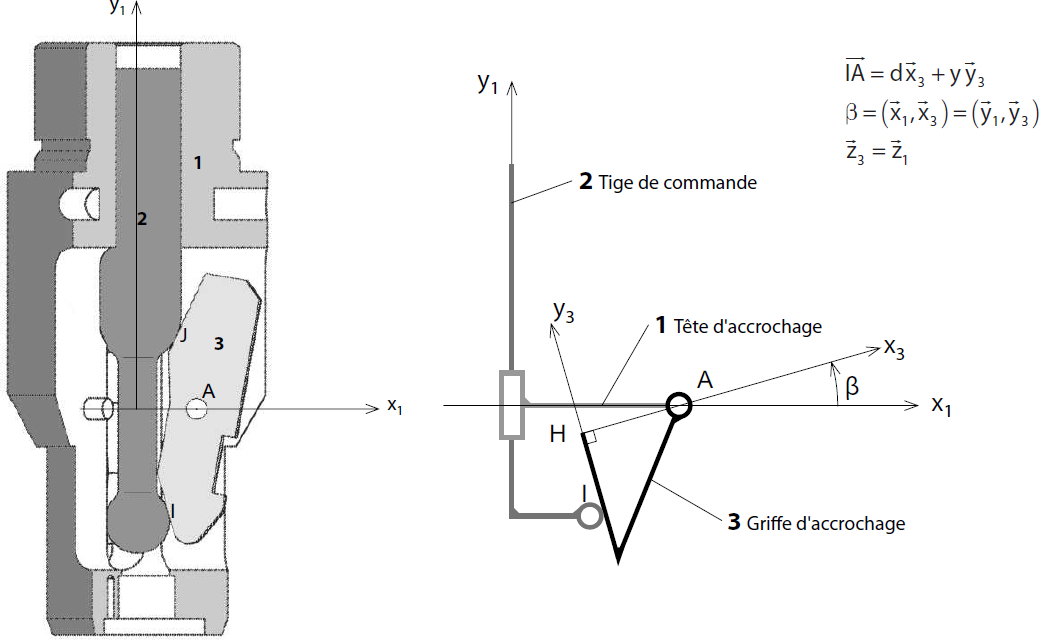
\includegraphics[width=.8\linewidth]{fig_01}
\end{center}
%\caption{Association en série d'une liaison pivot et d'une liaison  ponctuelle.}
%\end{marginfigure}
